\documentclass[12pt]{article}
\usepackage{amsfonts,amsmath,amssymb, listings}

\usepackage[utf8]{inputenc}
\usepackage{graphicx}
\usepackage{multirow}
\usepackage{xcolor}

\usepackage{threeparttable}
\usepackage{blindtext}


\usepackage[a4paper, total={6in, 8in}]{geometry}

\usepackage[numbered,framed]{matlab-prettifier}
%\usepackage{color}

%\setcounter{MaxMatrixCols}{10}

\def\stackunder#1#2{\mathrel{\mathop{#2}\limits_{#1}}}%

\newcommand{\fiid}{\func{i.i.d.}} % use this as in: X_i \stackrel{\fiid}{\sim} \func{Exp} \left( \lambda \right)
\DeclareMathOperator{\Norm}{N}

\newcommand{\platzo}{\vspace*{2cm}}
\newcommand{\platzt}{\vspace*{4cm}}

\newcommand{\findep}{\func{ind}}  % could use indep instead if ind, but 1st book uses ind.

\newcommand{\R}{\ensuremath{{\mathbb R}}}
\newcommand{\N}{\ensuremath{{\mathbb N}}}
\def\QATOP#1#2{{#1 \atop #2}}
\def\QTATOP#1#2{{\textstyle {#1 \atop #2}}}
\def\QDATOP#1#2{{\displaystyle {#1 \atop #2}}}
\voffset=-2.54cm\hoffset=-2.54cm \textheight27cm \textwidth17.0cm \topmargin0.5cm
\oddsidemargin2.00cm \evensidemargin2.00cm \unitlength1cm

\def\func#1{\mathop{\rm #1}}%
\def\dint{\mathop{\displaystyle \int}}%
\newcommand{\Ind}{\ensuremath{{\mathbb I}}} % indicator function
\newcommand{\E}{\ensuremath{{\mathbb E}}} % expected value
\newcommand{\Var}{\ensuremath{{\mathbb V}}} % variance

\setlength{\parindent}{0pt}

\usepackage{float}

\newfloat{Program}{thp}{lop}[section]
\floatname{Program}{Program Listing}

\begin{document}

\pagestyle{empty}

\bigskip

\begin{figure}[htp]
    \centering
    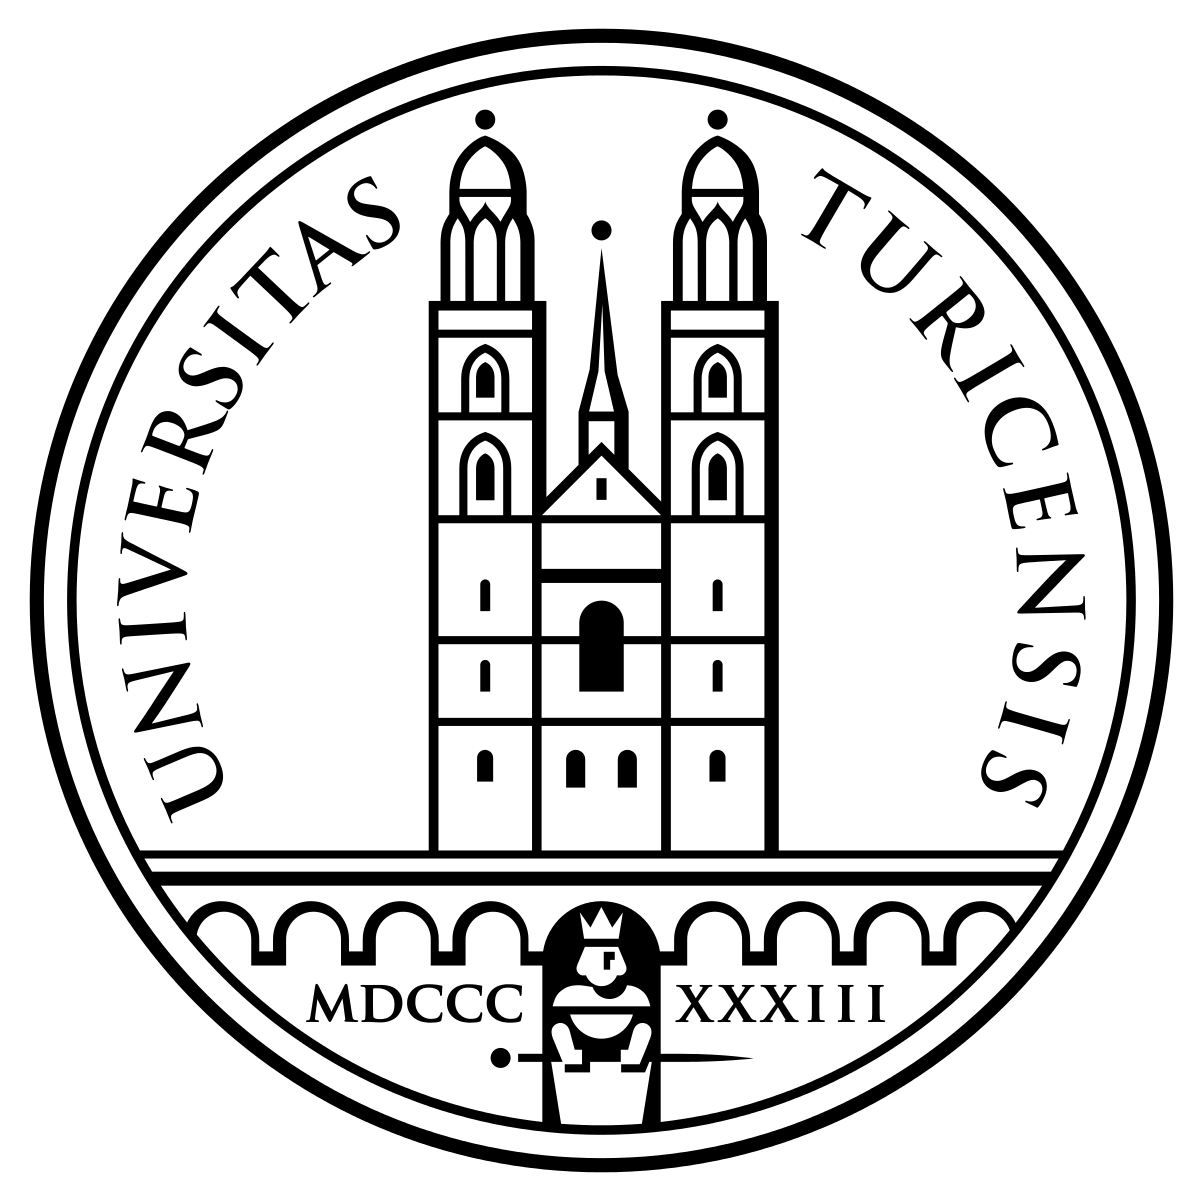
\includegraphics[width=4cm]{uzh logo 2.png}
    \label{fig:UZH}
\end{figure}

\begin{Large}
	\begin{center}
		\textbf{Digital Tools for Finance}
	\end{center}
\end{Large}

\vspace{2cm}

\begin{large}	
	\begin{center}
		\textbf{Effect of Interest Rate Changes on Cryptocurrencies - Research BTC} \vspace{0.1cm} \\ {Prof. Igor Pozdeev } \vspace{2cm} \\ \textbf{Matthias Olieslagers - 22714034}  \\ \textbf{Cameron Storey - Adapt stud nr} \\ 
        \textbf{Marc David Parker - Adapt stud nr}\\
        \textbf{Qian Chen - 21742226}\\
	\end{center}
\end{large}

\tableofcontents

\newpage

\bigskip
\section{Introduction}

\subsection*{Introduction}

The goal of this research report is to discover how changes in FED interest rates have an impact on the prices of cryptocurrencies (e.g. Bitcoin) \newline
The up-front hypothesis, based on our knowledge of the financial markets and backed by several resources (state resources) is that the higher the FED interest rate goes, the lower the crypto prices will drop, i.e. they have a negative correlation. In this report, an attempt will be made to  confirm (or invalidate) the hypothesis statement above. \newline
In the first section, the different data sources will be covered. What does the data exactly represent and why is it relevant to look into for this particular research. In the second part, the methodology will be laid out. Lastly, the results will be critically evaluated and interpreted and a final conclusion will be provided. 


\begin{Program}[!htb]
\begin{lstlisting}[style=Matlab-editor,basicstyle=\mlttfamily\footnotesize]
interesting if we wanna add the code 
\end{lstlisting}
\caption{Question 1 - Part 1}
\label{Question 1 - Part 1}
\end{Program}

\begin{Program}[!htb]
\begin{lstlisting}[style=Matlab-editor,basicstyle=\mlttfamily\footnotesize]
more code 
\end{lstlisting}
\caption{Question 1 - Part 2}
\label{Question 1 - Part 2}
\end{Program}


\section{Data}

\begin{Program}[!htb]
\begin{lstlisting}[style=Matlab-editor,basicstyle=\mlttfamily\footnotesize]
dummy
  
\end{lstlisting}
\caption{Question 2 - Part 1}
\label{Question 2 - Part 1}
\end{Program}


 




\



\newpage
\section{Methodology}

\end{document}
